\documentclass[tikz,border=10pt]{standalone}
% Scale s = 0.014981 cm/px, centred on ink bbox (cx=304, cy=183); y flipped.
\begin{document}
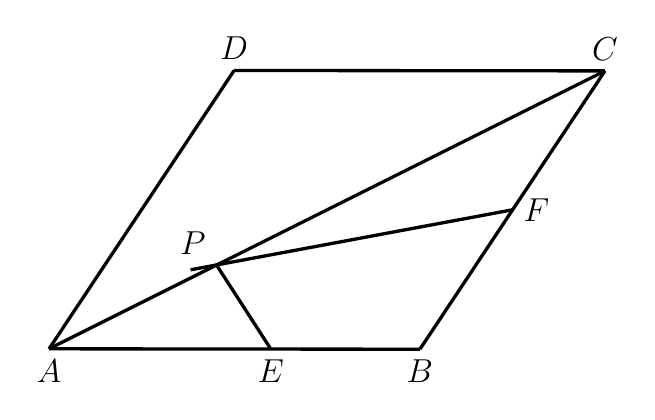
\begin{tikzpicture}[line width=1.2pt, line join=round]
  % Named coordinates (verified pixel points, converted to cm)
  \coordinate (C) at (3.5241678952494997,1.7630772399684698);
  \coordinate (D) at (-1.185309897239438,1.7684191834870628);
  \coordinate (A) at (-3.535633977317312,-1.766358915971033);
  \coordinate (B) at (1.1738438151716264,-1.7717008594896257);
  \coordinate (E) at (-0.7197133349746424,-1.769553004506332);
  \coordinate (F) at (2.351287137845049,-0.0008808667840721207);
  \coordinate (P) at (-1.4086416387347822,-0.70300277670447);
  \coordinate (Fext) at (-1.7387095562413102,-0.7630271880753351); % F extended through P

  % Segments
  \draw (C) -- (D);        % top
  \draw (A) -- (B);        % bottom, through E
  \draw (C) -- (A);
  \draw (C) -- (B);
  \draw (D) -- (A);
  \draw (F) -- (Fext);     % line F-P extended
  \draw (E) -- (P);

  % Labels
  \node[font=\fontsize{12}{14.4}\selectfont, above] at (C) {$C$};
  \node[font=\fontsize{12}{14.4}\selectfont, above] at (D) {$D$};
  \node[font=\fontsize{12}{14.4}\selectfont, below] at (A) {$A$};
  \node[font=\fontsize{12}{14.4}\selectfont, below] at (B) {$B$};
  \node[font=\fontsize{12}{14.4}\selectfont, below] at (E) {$E$};
  \node[font=\fontsize{12}{14.4}\selectfont, right] at (F) {$F$};
  \node[font=\fontsize{12}{14.4}\selectfont, above left] at (P) {$P$};
\end{tikzpicture}
\end{document}
% GEOAGENT_REPAIR_V1 c18a466396f54661 656bcd7032fb422a6f67ac4a8bf05a717e5682f0acbbf0e0a35dc5248a53da1d
